\chapter{Study 2: User Study}

Following the first study (See Chapter \ref{ch: chapter 3}), A laboratory study was conducted to evaluate user experience on different design patterns of music sequencers. Base on the previous work of evaluating music instruments, a questionnaire was designed to measure muscians experience (See Section \ref{subsec: questionnaire}).

\section{Method}
\subsection{Questionnaire}
\label{subsec: questionnaire}

Base on \citeauthor{Reference0}'s work, which developed a 80-item pool ordered by descending mean importance for questionnaire, 10 questions that scored the highest mark from 9 different categories were used in the user study (see Appendix \ref{app:Appendix A}).

\citeauthor{Reference0} indicated the following three criteria for musicians to perceive musical instruments:
\begin{flushleft}
  \qquad \qquad \quad\textbf{Experienced freedom and possibilities (EFP)}\\
  \qquad \qquad \quad\textbf{Perceived control and comfort (PCC)} \\
  \qquad \qquad \quad\textbf{Perceived stability, sound quality and aesthetics (PSSQA)}\\
\end{flushleft}
\textit{EFP} as the predominent facet, mainly targets at evaluating the musicianship and expressivity of music instruments. For example, questions like\textit{\textquotedblleft{The instrument allows me to express myself.}\textquotedblright} are used to decide whether the instruments can let muscians to express themselves; \textit{PCC} is used to assess the controbility of the music instruments. Questions such as \textit{\textquotedblleft{I can control the sound appropriately.}\textquotedblright} are setted to identify how well the musicians believed they can control the instruments; \textit{PSSQA} is the most unique facet which analyses the quality of the instruments from the material, the sound and the apperience perspectives. For instance, questions like\textit{\textquotedblleft The instrument pleases me sound-wise\textquotedblright} test the sound quality of the instrument. The above three interrelated facets construct the framework of MPX-Q questionnaire.

\begin{table}
  \caption{Items in the questionnaire with thier factor and category(ordered by descending mean importance)}
  \label{tab: questionnaire}

  \begin{tabular}{ |p{1.2cm}|p{2.5cm}|p{9.2cm}|p{0.6cm}|}
   \multicolumn{4}{l}{} \\
   \hline
   Factor & Category  & Item  & $\mu$ \\
   \hline
   EFP & Creativity & The instrument allows me to be creative & 6.25\\
   & Enjoyment &  I have fun playing the instrument & 6.08\\
   & Expressiveness & The instrument allows me to express myself & 6.06\\
   \hline
   PCC & Conformance & The instrument responds well to my actions & 6.23\\
   & Control & I can control the sound appropriately & 6.04\\
   & Engagement & The instrument allows me to be engaged when I'm playing it & 5.98\\
   & Engagement & I feel the urge to play the instrument again & 5.79\\
   & Play Comfort & I can recognize that the instrument responds well to my playing & 5.85\\
   \hline
   PSSQA & Stability & I can rely on the instrument when playing it & 6.21\\
   & Sound Quality & The instrument pleases me sound-wise & 6.02\\
   \hline
  \end{tabular}
  % \small should be a caption
\end{table}

\bigskip

Follow the framework of MPQ-Q questionnaire, 10 questions from 3 factors were implemented in our questionnaire(see Table \ref{tab: questionnaire}). For each factor, only the items score the highest mean importance value in the certain category were picked. Under the EFP factor, we focused at the creativity, enjoyment and expressiveness of the music sequencer. The reason for this, it's because we want to figure out whether the design of the interface is encouraging musicians to explore new possibilities and inspiring musicians' creativity. As for the PCC, items associate with conformance, control and engagement are chose. The reason behind this is when musicians performing on instruments there are a lot of physical interaction between musicians and instruments, whether the musiciain feel conformance and engagement have impact on their overall satisfaction. For items under PSSQA, we only look at the stability and sound quality. Because the more stable of the music sequencer the more confident musicians can rely on it. Same with the sound quality, only the instrument that can satisfy the muscian is able to please the audience.

\subsection{Participants}

In total, twenty participants with different music background were invited and took part in the user study. Fifteen of them are male and five are female. All the participants have at least one year training on music and master at least one instrument. Two participants are semi-professional musicians who have spend more than 10 years on performing and music making. One are currently teaching music in the middle school. The remaining musicians play musical instruments mainly because their parents forced them to do when they were children, however, they were all greatful that they have learned music and still practise the instrument in their spare time.

\bigskip
\begin{figure}[h]
  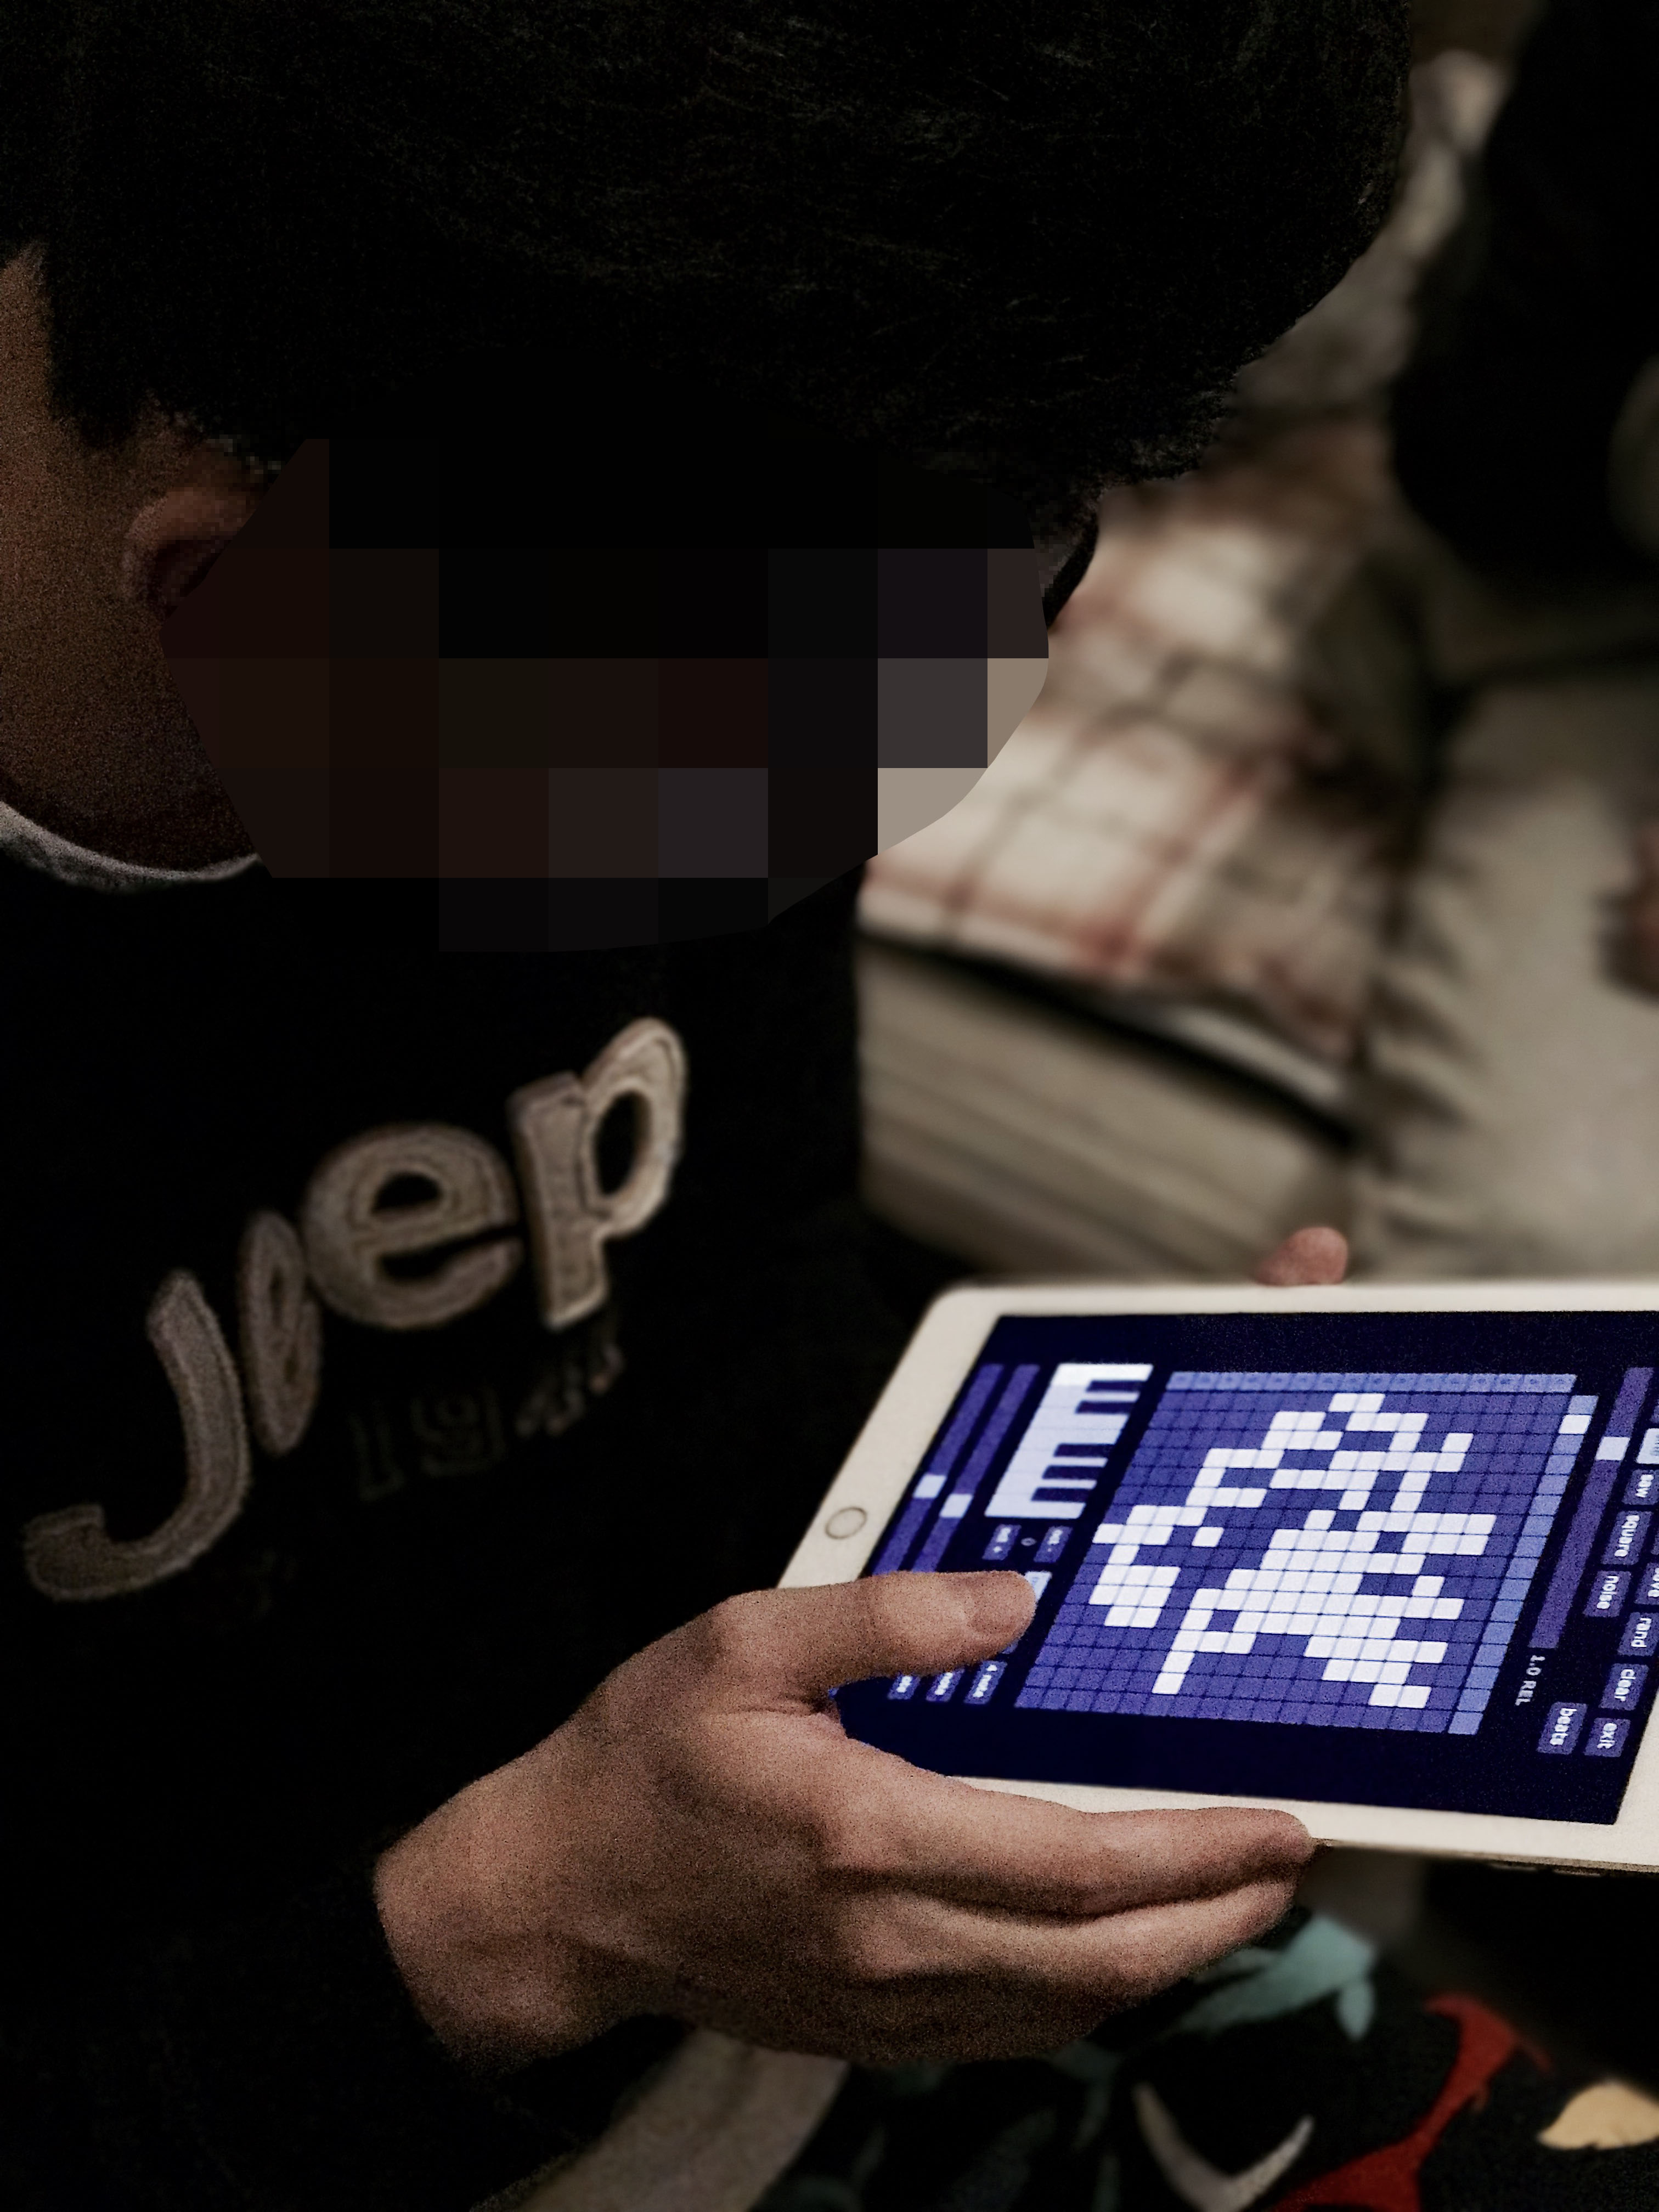
\includegraphics[width=6cm]{images/Participant}
  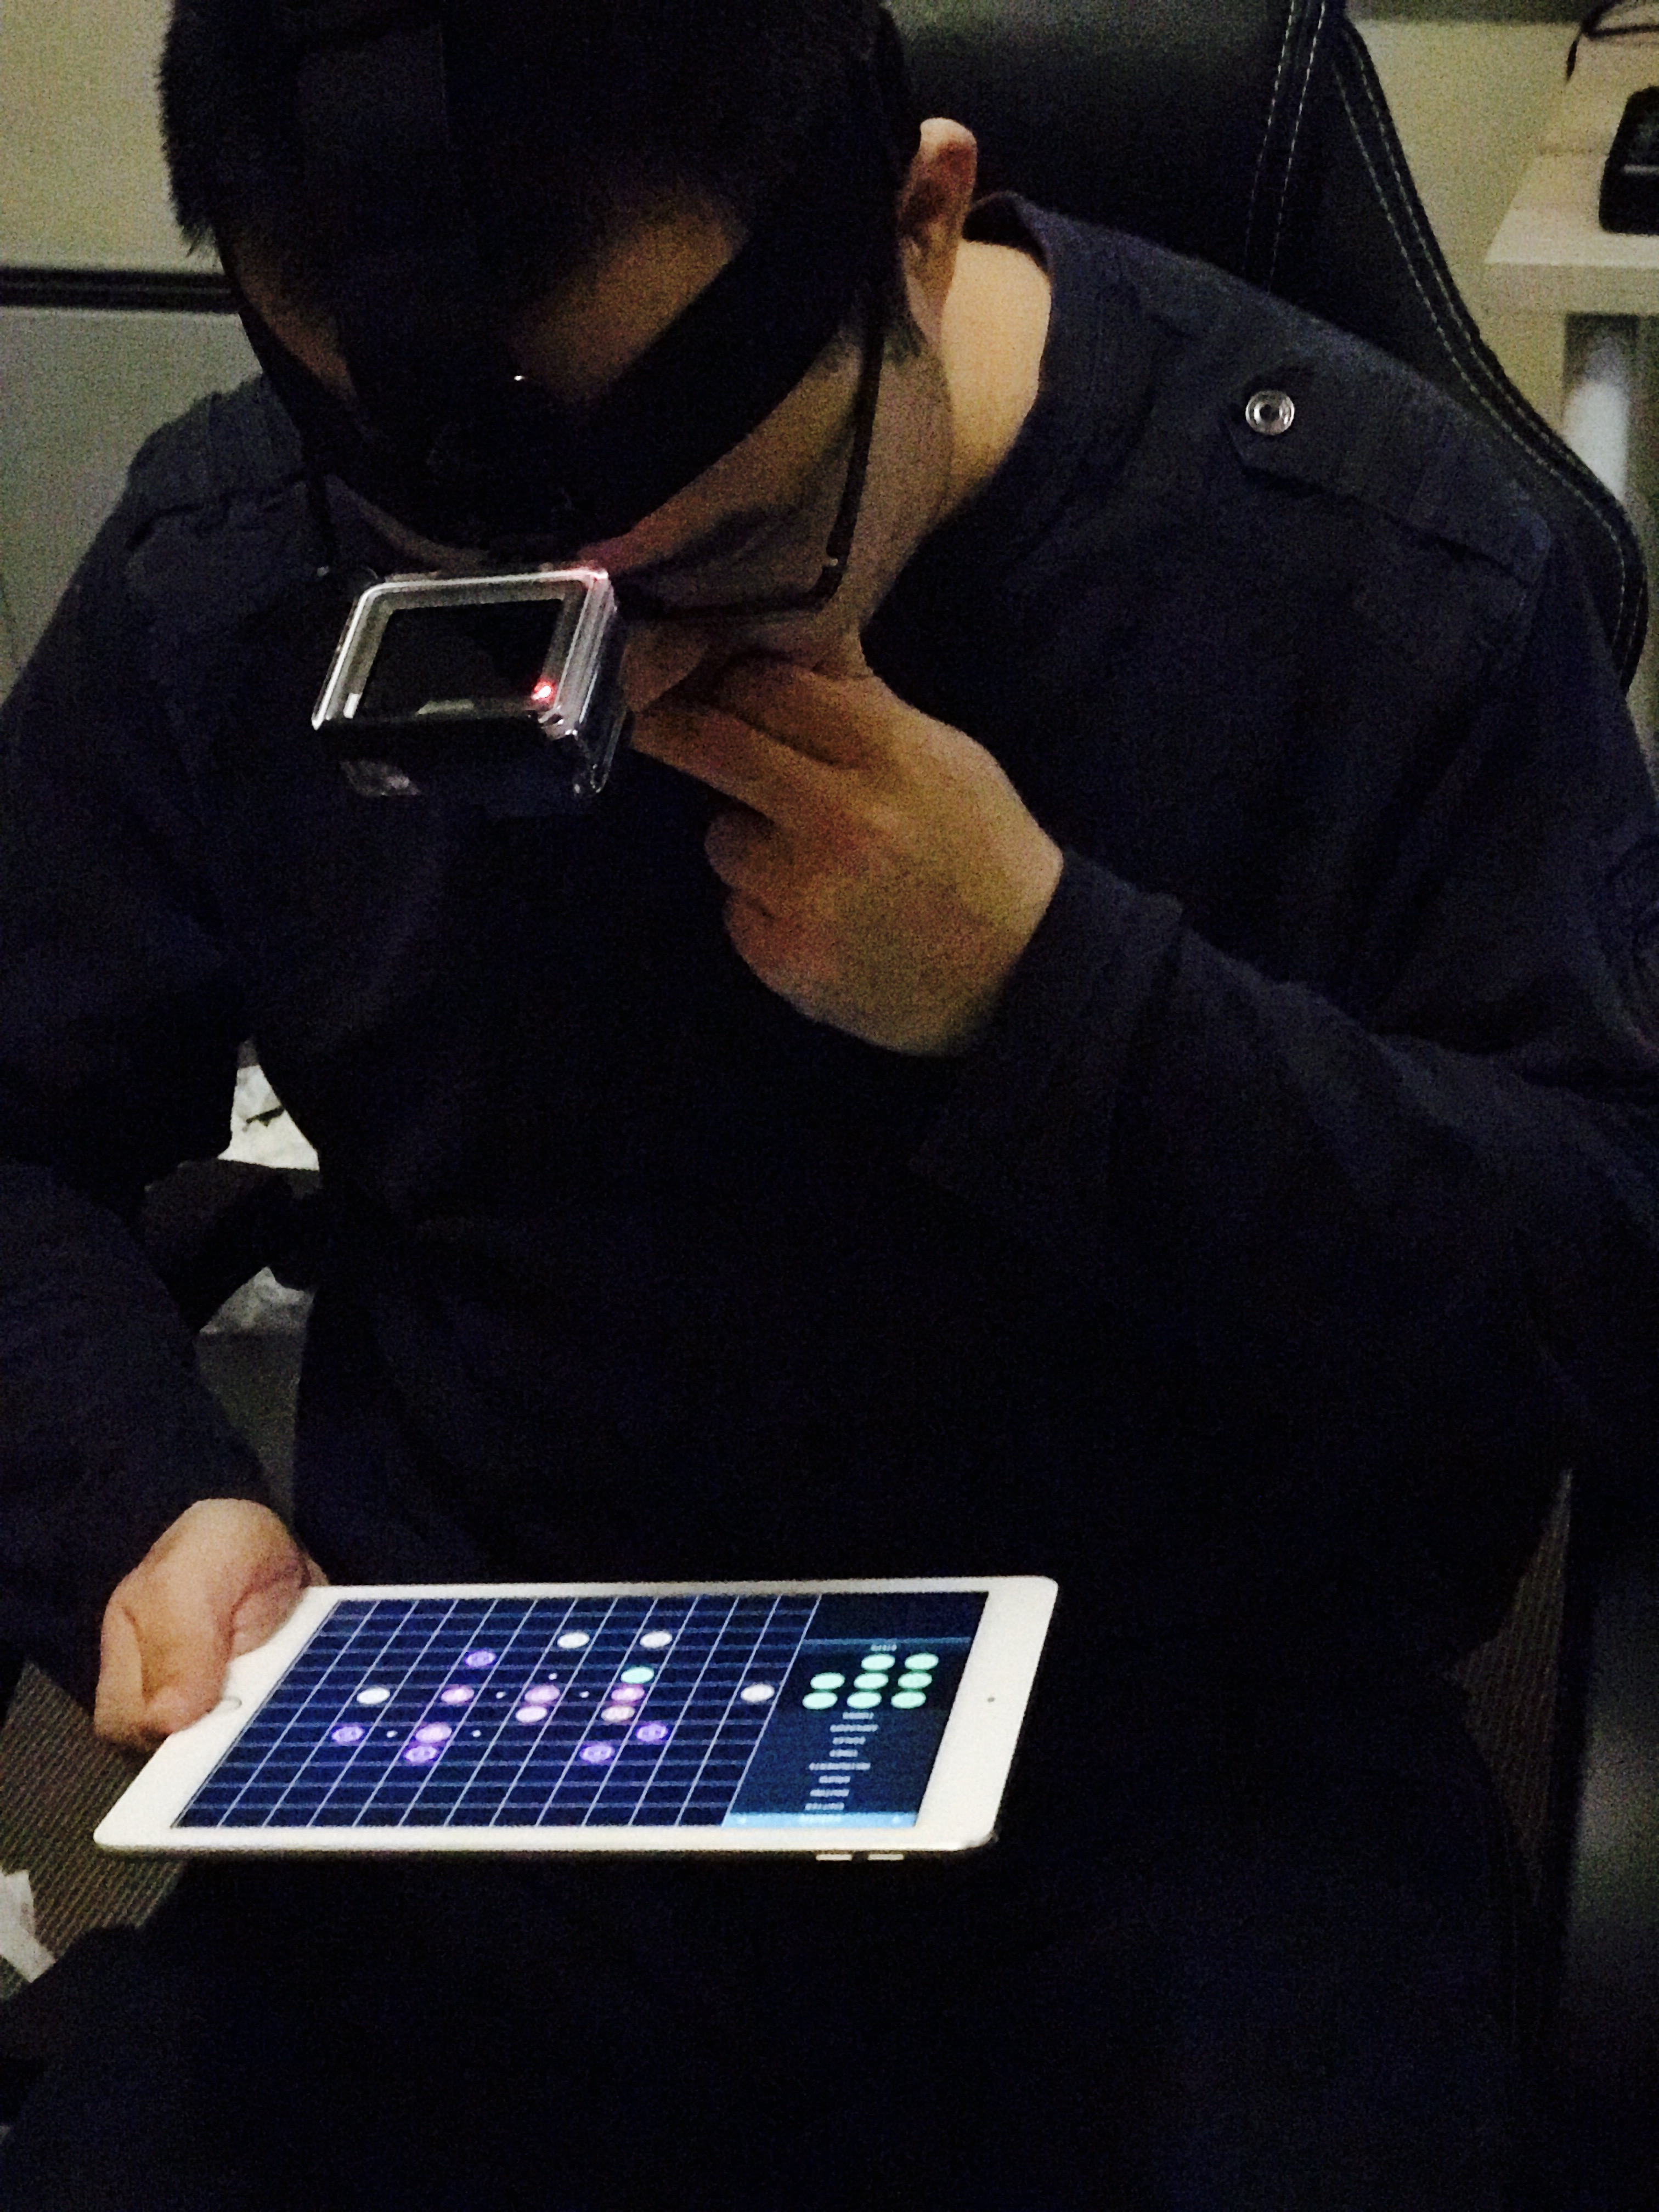
\includegraphics[width=6cm]{images/Participant2}
  \centering
  \caption{Participants test on the music sequencer on iPad}
  \label{fig: participant}
\end{figure}
\bigskip


Four of them have learned more than one instrument. One have learned more than five different instruments. The popular pick of instruments are piano and guitar. Ten participants have learned to play piano and three of them have over five years experience. Seven participants have learned guitar and still play guitar occasionnally. Other instruments are drums, violin and flute. Three participants have experience playing drums. Two have learned to play violin. Two have learned some flute many years ago. But only 15\% had experience on electronic music before and had played on music sequencer on the laptop.

\subsection{Interview}

Participants were intervied at the end of the user study. The main purpose of the interview is to find out the reason behind their decision on the questionnaire. Besides, the music background of participants such as \textit{\textquotedblleft{how many years of music training}\textquotedblright} were recorded for further analysis.

In order to acquire the deeper reason, all the interview followed the same procedure: 1) Since the majority of the participants did not know music sequencer before, they were asked to describe the similarities among the three different music sequencer applications, and then defined what is music sequencer. which was designed to help them to form a general idea of music sequencer. 2) After that, interviewees were asked to choose their favourite application based on different scenario. Also, the interviewee needed to give reasons why certain music sequencer application was better than another. 3) In the final step, all the questions shifted to an abstract level, where they were asked whether music sequencer application on iPad were an instrument ,and what features that made them thought it is or it is not an instrument.The interviews were recorded on video and audio based on the participants agreement. The recording lasted between 10 to 20 minutes.

\section{Results}

\subsection{Quantitative Results}
From the questionnnaire, in total 600 satisfaction items were extracted. A satisfaction item is a number between one to five, which represents interviewee's degree of agreement over one certain statement. The higher number a statement scored means the more the interviewee agreed with it. The raw data was first recorded on an Excel workbook. Thanks to my supervisor Ben, who offer his help on data visualisation, the tedious numbers come to live. An overview of the participants response on the 10 questions with the selected music sequencer application is given in Figure \ref{fig: questionnaire}.

\bigskip
\begin{figure}[h]
 \centering
 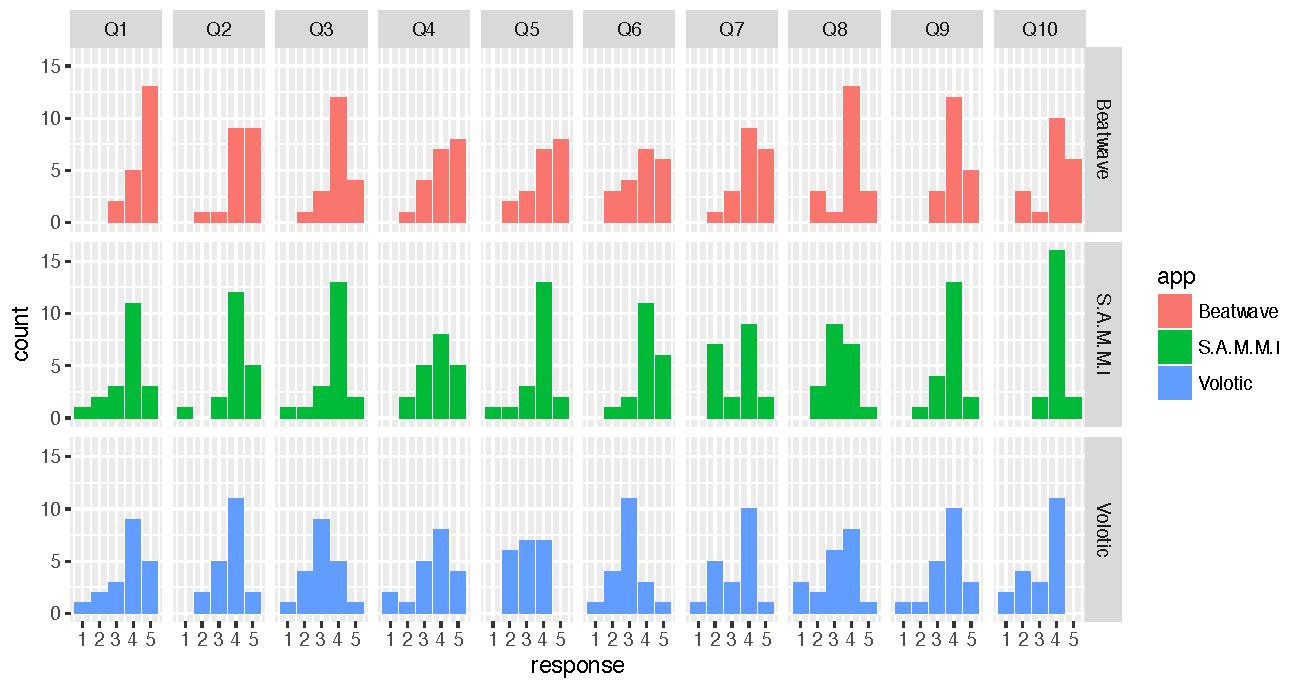
\includegraphics[width = \textwidth]{images/questionnaire-responses.pdf}
 \caption{Overview of participants response over three music sequencer application}
 \label{fig: questionnaire}
\end{figure}

In Figure \ref{fig: questionnaire}, x-axis is divided into 10 columns which relatively represent 10 questions in the questionnaire. At the bottom of each column, there are numbers from one to five, which are used to measure participants agreement over the question. The y-axis consist of three major row. In each row, the height of each bar denote the total amount of participants who shared the same opinion. Take the top-left section for example, for music sequencer \textit{Beatwave}, thirteen participants strongly agreed on question one, five people just agreed on the statement by giving four marks and two people gived neutral comments.

\bigskip
\begin{figure}[h]
 \centering
 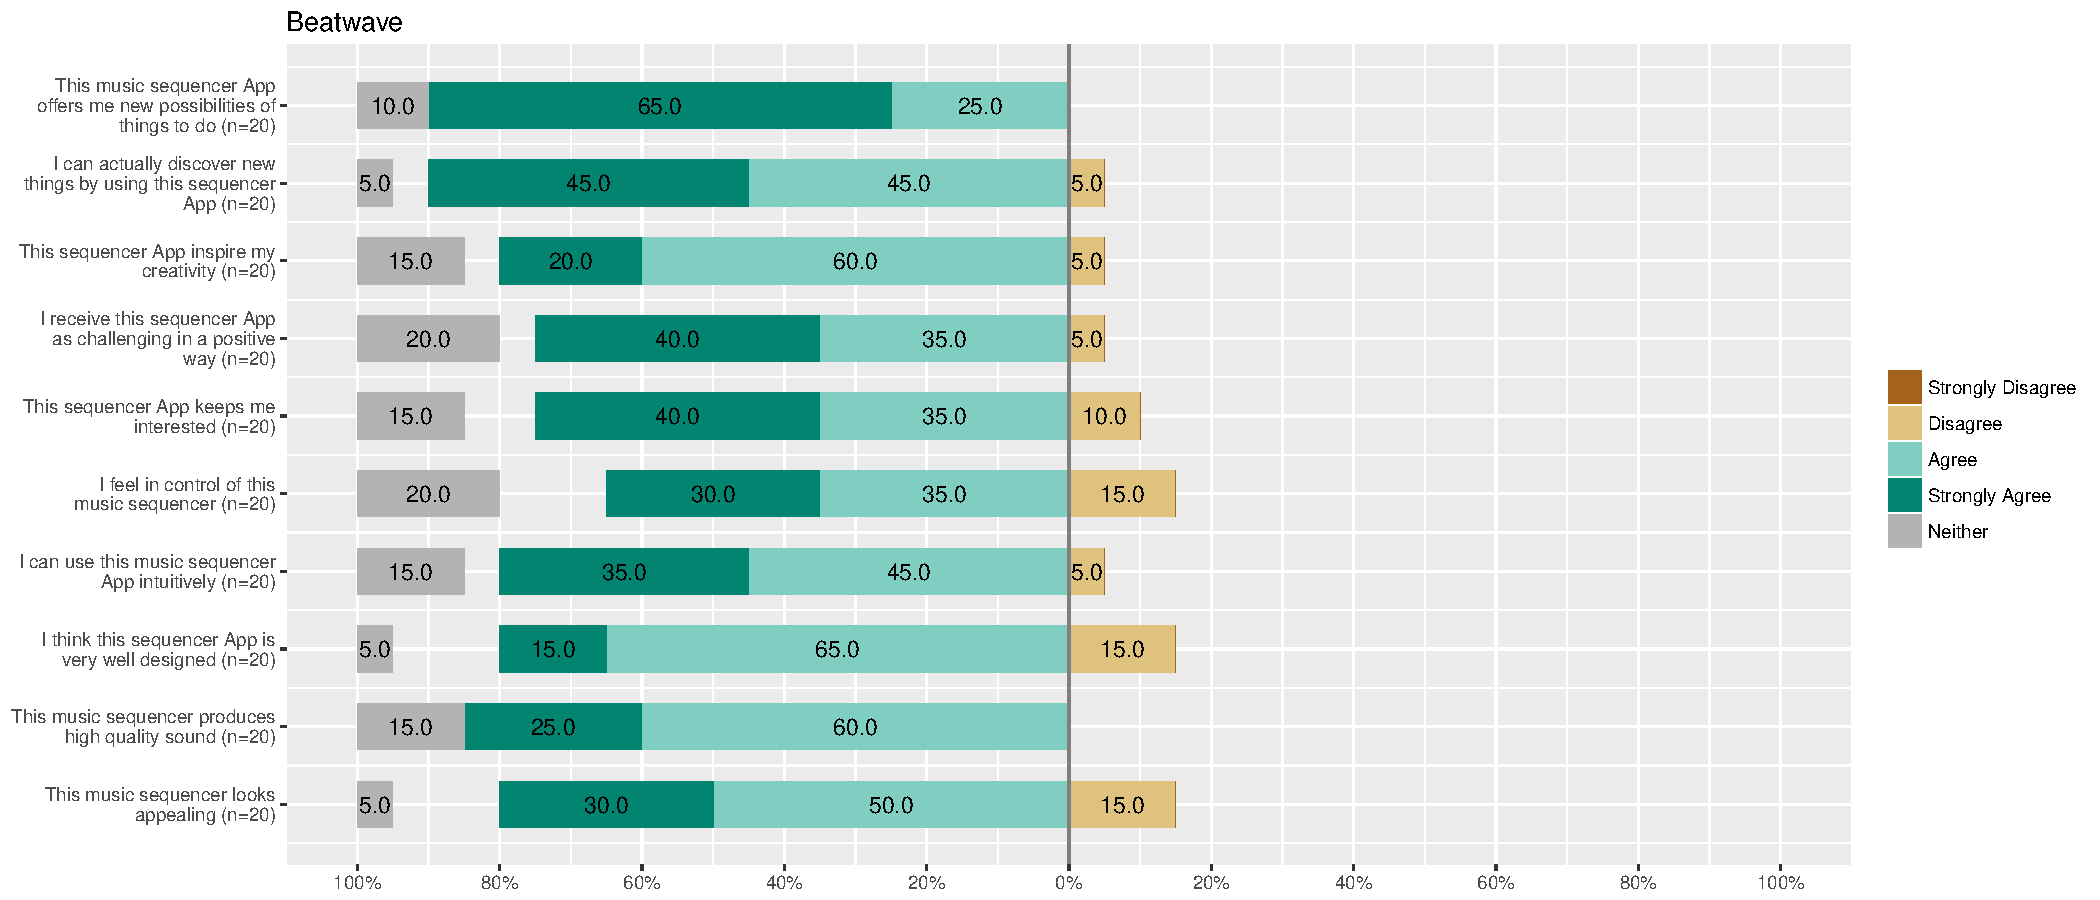
\includegraphics[width = \textwidth]{images/Beatwave.pdf}
 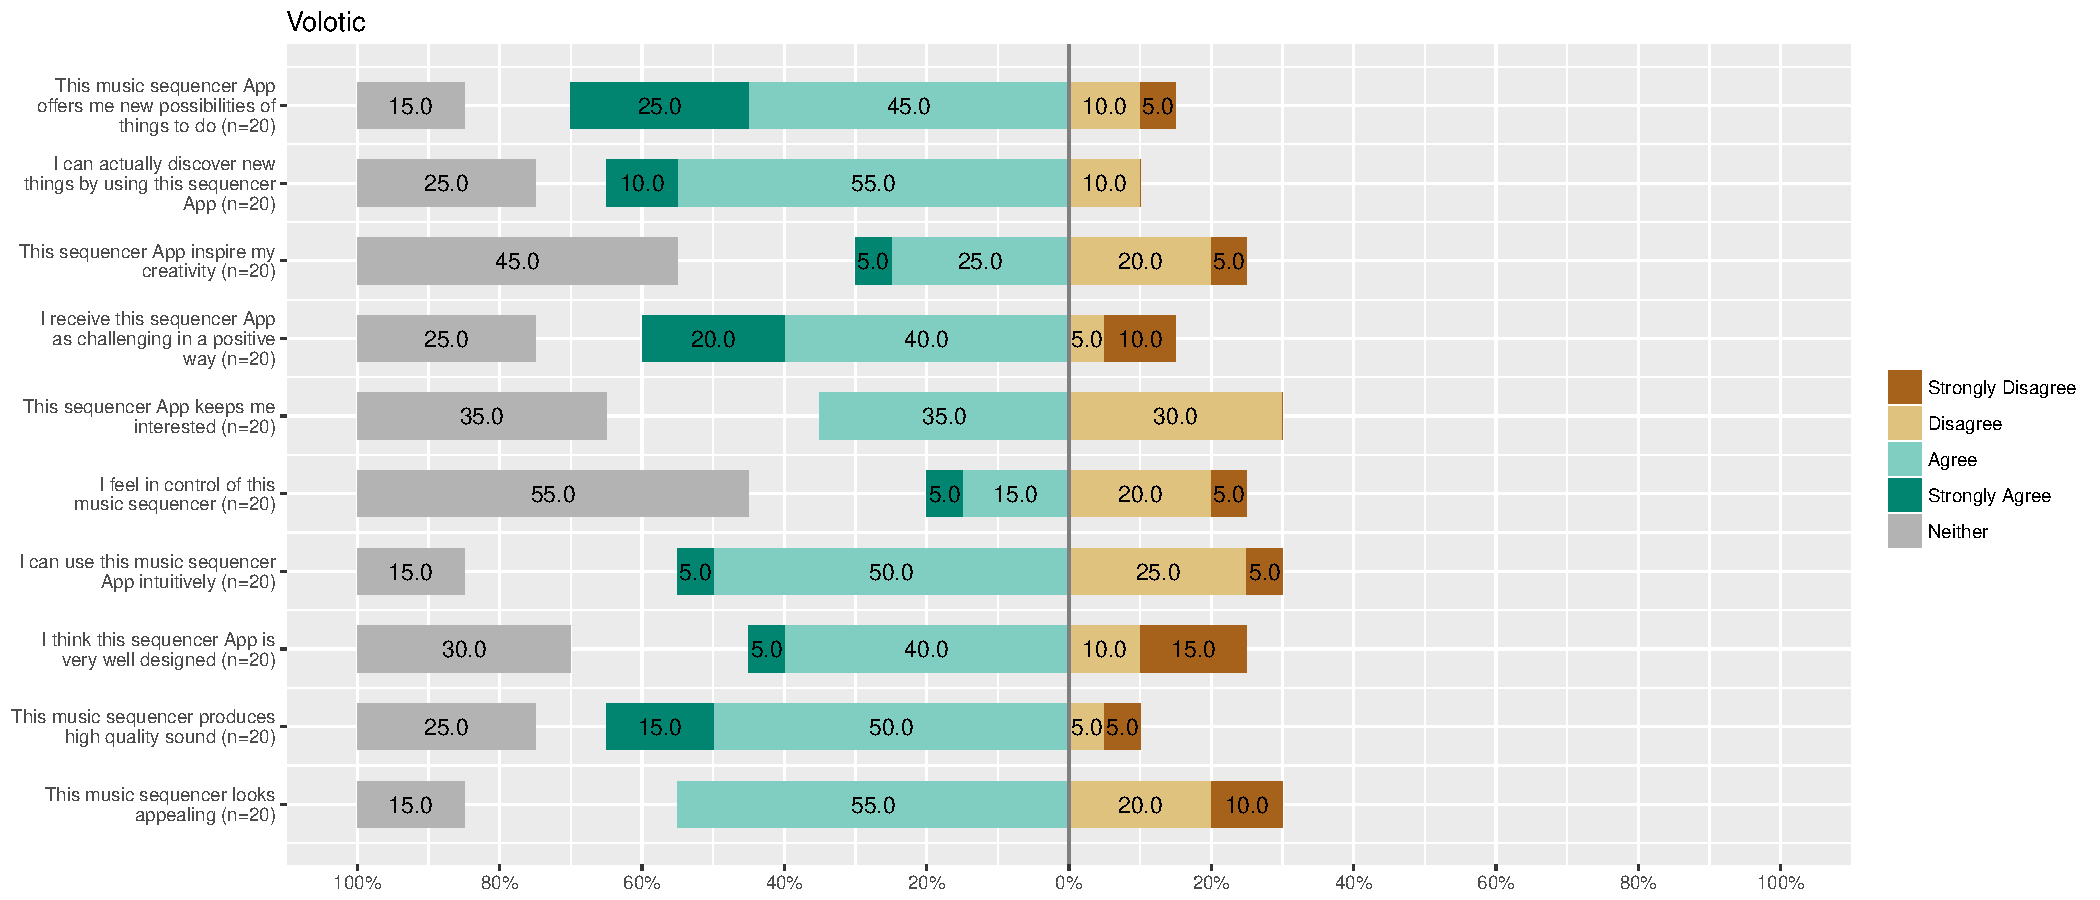
\includegraphics[width = \textwidth]{images/Volotic.pdf}
 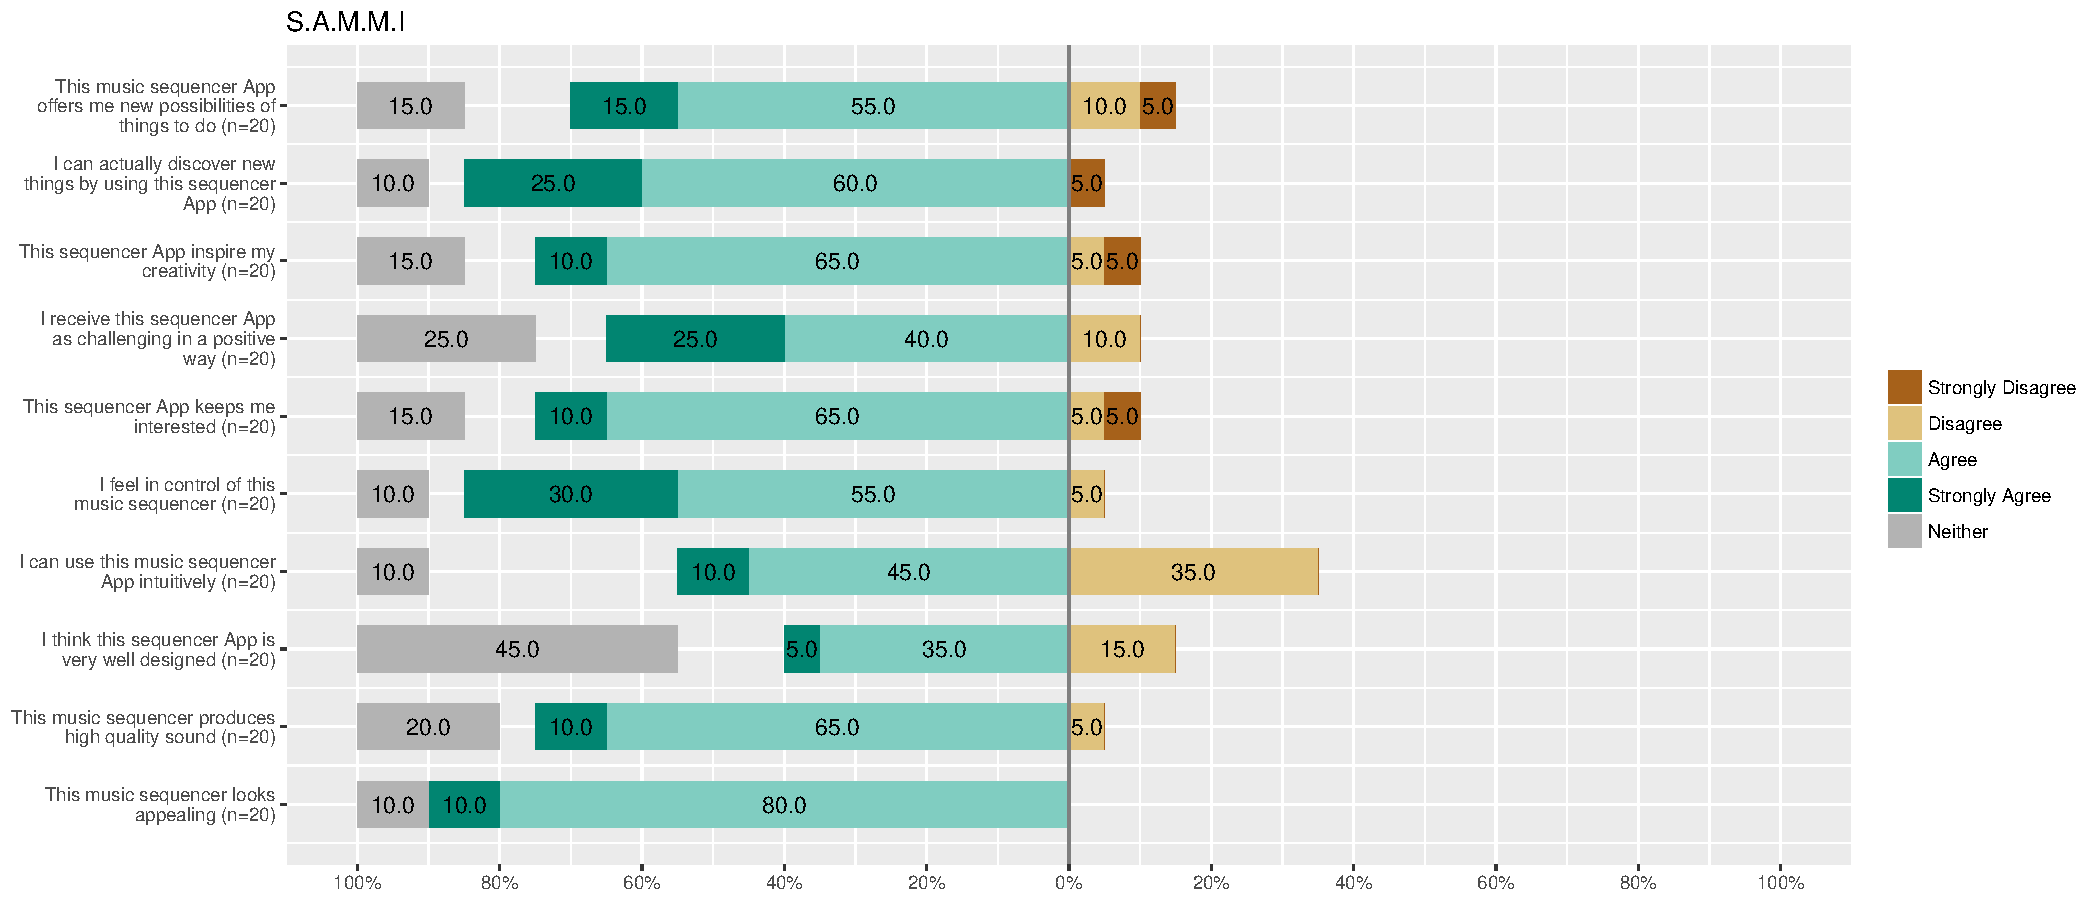
\includegraphics[width = \textwidth]{images/SAMMI.pdf}
 \caption{Participants response on Beatwave, Volotic and S.A.M.M.I}
 \label{fig:result_response}
\end{figure}
\bigskip

The detailed information of participants opinions over each application is given in Figure \ref{fig:result_response}. For each question on the left, there is a relative bar shows the percentage of the five likert scale. For instance, the first row in the top shows 65$\%$ participant strongly agreed with the corresponding statement on the left side, meanwhile, 25$\%$ people just agree with it. And 10$\%$ people remained neutral.

\subsection{Qualitative Results}

The result in this section is based on the information extracted from the interview. According to participants music-training background and the type of instruments they mainly used, we seperated the musicians into three groups: Group One (Playing traditional instruments but with less than three years formal music trainning), Group two (Playing traditional instruments but with more than three years formal music trainning), Group three (Playing electronic instruments and had more than three years formal music trainning). The reason why we don't have a group for musicians who play electronic instruments but less than three years formal music training is all the participants who play electronic instruments has many years experience in playing traditional instrument before.

\textbf{Group One:} Participants in this group have less experience in music in general, comparing with other two groups. They found \textit{S.A.M.M.I} was very easy to use becasue of the intuitive design of interface. Although \textit{S.A.M.M.I} didn't provide much options in terms of different sounds and adjustment on the sound effect, it was complex enough for them to discovery most of the possibilities. Besides, thanks to the annotation of different pitch, \textit{S.A.M.M.I} is the only application that they were able to create a short piece of melody, such as \textquotedblleft{Song of Joy}\textquotedblright and \textquotedblleft{Mary Had a Little Lamb}\textquotedblright.

The comments on \textit{Beatwave} were mainly focused on the layout of different tracks. They agreed combining severl layers of music together was definitely an improvement, but this design pattern made it more difficult to control comparing to the single-track interface design of \textit{S.A.M.M.I}. Furthermore, participants in Group One believed the visual effect of \textit{Beatwave} gave them a positive feedback. The rippling effect of the current note helped them tracked down the progress of the music.

\textit{Volotic} was recognized as the most difficult application to create music. Most participants in this group thought \textquotedblleft{It's more like a game rather than an instrument}\textquotedblright. But they still thought it was a very good practice and could potentially used to help kids generate interest in music.   


% \bigskip
% \begin{table}
%   \caption{Participants response on three different applications}
%   \label{tab: interview}
%
%   \begin{tabular}{ |p{2cm}|p{3.5cm}|p{3.5cm}|p{3.5cm}|}
%    \multicolumn{3}{l}{} \\
%    \hline
%    Apps &
%    Traditional Instrument(less than 3 years trainning) & Traditional Instrument(more than 3 years trainning)  & electronic Instrument(more than 3 years trainning) \\
%    \hline
%    Beatwave & The design of multitrack
%    \hline
%
%    \hline
%
%    \hline
%   \end{tabular}
%   % \small should be a caption
% \end{table}
% \bigskip
% % \small should be a caption
